\documentclass[a4paper]{article}
\usepackage[english]{babel}
\usepackage[T1]{fontenc}

\usepackage[a4paper,top=3cm,bottom=2cm,left=3cm,right=3cm,marginparwidth=1.75cm]{geometry}

\usepackage{natbib}
\usepackage{url}
\usepackage[utf8x]{inputenc}
\usepackage{amsmath}
\usepackage{listings}
\usepackage{float}
\usepackage{graphicx}
\graphicspath{{images/}}
\usepackage{parskip}
\usepackage{fancyhdr}
\usepackage{vmargin}
\usepackage[titletoc]{appendix}
\usepackage{subcaption}

\usepackage[ruled]{algorithm2e}

%%\setmarginsrb{3 cm}{2.5 cm}{3 cm}{2.5 cm}{1 cm}{1.5 cm}{1 cm}{1.5 cm}

\title{Unity Game}						% Title
\author{Group 7}
\date{\today}											% Date

\makeatletter
\let\thetitle\@title
\let\theauthor\@author
\let\thedate\@date
\makeatother

\pagestyle{fancy}
\fancyhf{}
\rhead{\theauthor}
\lhead{\thetitle}
\cfoot{\thepage}

\begin{document}

%%%%%%%%%%%%%%%%%%%%%%%%%%%%%%%%%%%%%%%%%%%%%%%%%%%%%%%%%%%%%%%%%%%%%%%%%%%%%%%%%%%%%%%%%

\begin{titlepage}
	\centering
    \vspace*{0.5 cm}
    
\includegraphics[width = 0.4\textwidth]{IST_A_RGB_POS.png}\\[0.1 cm]	% University Logo
	\textsc{\Large 3D Programming}\\[0.5 cm]				% Course Code
	\textsc{\large Assignment \#3}\\[0.8 cm]				% Course Name
	{ \huge \bfseries \thetitle}\\[1.5 cm]
	
	\begin{tabular}{l @{\hspace{2 cm}} r}
    	\large \emph{Group 7:} & \large \emph{Student Number:} \\ [0.5 cm]
		\large Luís Fonseca & \large ist79770 \\
		\large Ricardo Fonseca & \large ist90862 \\
	\end{tabular}
    
	 
	\vfill
	
\end{titlepage}

%%%%%%%%%%%%%%%%%%%%%%%%%%%%%%%%%%%%%%%%%%%%%%%%%%%%%%%%%%%%%%%%%%%%%%%%%%%%%%%%%%%%%%%%%

\tableofcontents
\pagebreak

%%%%%%%%%%%%%%%%%%%%%%%%%%%%%%%%%%%%%%%%%%%%%%%%%%%%%%%%%%%%%%%%%%%%%%%%%%%%%%%%%%%%%%%%%
\section{Game Overview}
The goal of this assignment was to create a 3D game using the Unity game engine while focusing on global illumination. The game was developed using Unity 2017.3.1.

Our game mechanics and aesthetics take inspiration from the Tron movies. The player holds a disc similar to the identity disc in Tron which can be thrown to destroy obstacles and enemies thus earning score points. The player loses if it's health reaches 0 or it falls out of the map. To win, the player must reach the white highlighted area.

\section{Implementation}

\subsection{3D Scene}
The game scene is composed mainly by regular geometry to fit the  overall game theme. There are two spaces in the level, indoors and outdoors, which have different textures to differentiate between the two. The light emitted from the floor and a directional light illuminate the outdoor space. On the other hand, the indoor scene is lit by several different colored point lights. 

To navigate the scene, there are autonomous yellow platforms, moving up and down, that allows the player to reach higher places since it cannot jump.

\subsection{Game mechanics}

	The game uses the first person shooter perspective with the main camera defined inside the player game object.
   
	\subsubsection{Player}
    The player is defined by a capsule collider and a rigidbody which allows the the character to hit other objects and be affected by gravity.
    
    
    
    The character control is defined in three scripts: \textit{PlayerController}, \textit{PlayerMotor} and \textit{CameraAim}. In order to move the player, pick objects or shoot the disc, the \textit{Update} function in \textit{PlayerController} checks the user input. If the user moves the mouse  or moves the character, we calculate the player transform and the camera rotation and move each game object accordingly in \textit{PlayerMotor}. The first script also allows us to control the inventory by picking objects ("P" button) or selecting items from the inventory ("1,2,3" buttons). The object pickup action utilizes rays casted from the camera. If the ray intersects an interactable object, then depending on the distance, it focus that object and the player is able to pick it up. The mouse button 1 throws the disc if it's in the players possession or retrieves it to the hand otherwise.
     
     \subsubsection{Disc}
	The disc serves as a weapon just like any other first person shooter. We define the disc behaviour in the \textit{DiscController} script. Since the disc is defined by a cylinder collider and a rigidbody, we define two states: when its on the players hand it can't interact with the player's collider and when is thrown it bounces of the scene objects with colliders. The script allows us to set the hit damage, the speed, the player's catch radius and the maximum throw distance of the disc. When the disc is thrown, the collider listens to a  trigger event in order for the player to catch the disc when it is in its radius.
    
    Different types of discs were made into prefabs where different behaviour was possible by labeling them with different tags.
    
	\subsubsection{Inventory}
     Throughout the scene there are a few discs that were defined with \textit{Interactble} behaviour. Whenever the player is close enough and looking at the objects, they are highlighted which means they can be picked up. The player starts with a normal disc in the inventory and is able to pickup the ice and fire discs during gameplay. The ice and fire discs differ from the normal not only on the textures but also on behaviour. The ice disc inflicts less damage but freezes the enemies motion temporarily. As for the fire, it deals damage over time.
          
    \subsubsection{Enemies and Obstacles}
    
     Enemies are turrets that fire bullets towards the main character. An enemy is defined by two colliders. One collider is used to trigger the turret target. \textit{OnTriggerEnter} sets the player as the target and starts shooting bullets at him and \textit{OnTriggerExit} sets the turret to an idle state. The other collider checks if it's hit by a disc object and decreases the enemy health according to the disc type. At certain stages, the enemy's health triggers different particle systems to indicate its life status.
     
     We also define moving walls with rigidbodies as obstacles where each one is contained inside a collider. The movement is defined by trigger events: when the wall is inside the collider, we add a force to the rigid body. On the other hand, when the wall exits the collider, we change the direction of the force. Doing so keeps the wall moving back and forth perpetually.
     The walls rigibodies are frozen on the y and z axis to obtain movement only in x direction.
     
     
    \subsubsection{Score System and Level Completion}
   The current score is defined by a small script which is updated when the player destroys an enemy. To end the game, the player dies (either by falling out of the map or losing all the health) or reaches the game completion zone.
   This prompts the end screen menu with a different message according on how the game ended.
   The current score, players name and game status are kept in the \textit{PlayerPrefs} so the information isn't lost when there is a scene change. To keep records from all sessions, the current session information is saved in a persistent .json file.

\subsection{UI}
	\subsubsection{Heads-Up display}
    The heads-up display is divided in: current score on the left , the crosshair in the center and  the health bar, mini-map and inventory on the right. All the HUD elements were created using Unity's UI elements.	   
   The health bar is composed by two images and text that shows the player health percentage. Whenever the player takes damage, we recalculate the current health and maximum health ratio and scale the bar fill on the x axis. To render the mini-map, we use an orthographic camera that follows the player in the x and z coordinates. The camera saves an image of every frame as output which is used as source for the screen UI element.
   The inventory bar is composed by different slots which one containing one type of disc. When the player picks a new disc, the first empty slot is filled with a image according to the type of disc.   
    
  	\subsubsection{Main Menu}
    Our main menu was created on a new scene using Unity's UI. The main screen is composed by buttons that lead to different sub-menus, e.g the Help Menu. The buttons behaviour were implemented using the \textit{OnClick} function where we hide the main screen menu and enable the game object associated with the sub-menu. Using the same functionality, we implement the return buttons in the sub-menus.
   
   Pressing play directs us to a screen with a text input field used to define the player's name. When finished, the player presses enter to load the level and start the game. 
    
  	\subsubsection{End Menu}
    Much like the Main Menu, the end menu was created on a different scene. It contains a button that allows the user to return to the main menu and a table with the best scores.
    On top of the screen, we have a message that changes according to how the game ended ("\textit{Game Over!}" or "\textit{Level Complete}!"). The current score is displayed below that message and it's only recorded if the player is able to complete the level.
    
    
\subsection{Visual Effects}
	
    All the visual effects were obtained using built-in shaders from Unity and using the Post Processing stack.

	\subsubsection{Particle Systems}
    
    Two types of particle systems were used in the game: smoke and explosions. The smoke (fig.3a ) changes to a darker color over lifetime according to the enemy's damage. The explosion (fig.3b) is triggered by the enemy's death. Both particle systems were obtained from the unity asset store and use textures with normal maps with different sizes over the lifetime. The explosion uses a point light for a more vivid effect.
    
    \subsubsection{Bump Mapping}
    We implemented normal mapping on the stone walls and floor of the indoor section of the scene. In fig.4, we see a block of stone illuminated by the emissive floor and the sun (direct light) where the normal maps makes it look like an irregular surface.
    
    \subsubsection{Lightmap and Ambient Occlusion}
    In order to allow light mapping, we set all the game objects except the enemies to static objects. In Unity lighting settings, we enable the baked global illumination option and set to baked indirect mode. We also set ambient occlusion in Unity lighting settings.
    
    \subsubsection{Reflection Probes}
    We use reflection probes to generate cubemaps that are used by the scene walls with reflective materials. As we can see in fig.7, the cube material reflects the skybox.
    
    \subsubsection{HDR Bloom}
    Using a free asset from the asset store, we enable bloom in order to obtain the emission effect from the disk and floor materials.
    



\newpage
\appendix
\section{Images}
\subsection{User Interface}
  \begin{figure}[H]
      \begin{subfigure}[b]{0.33\linewidth}
          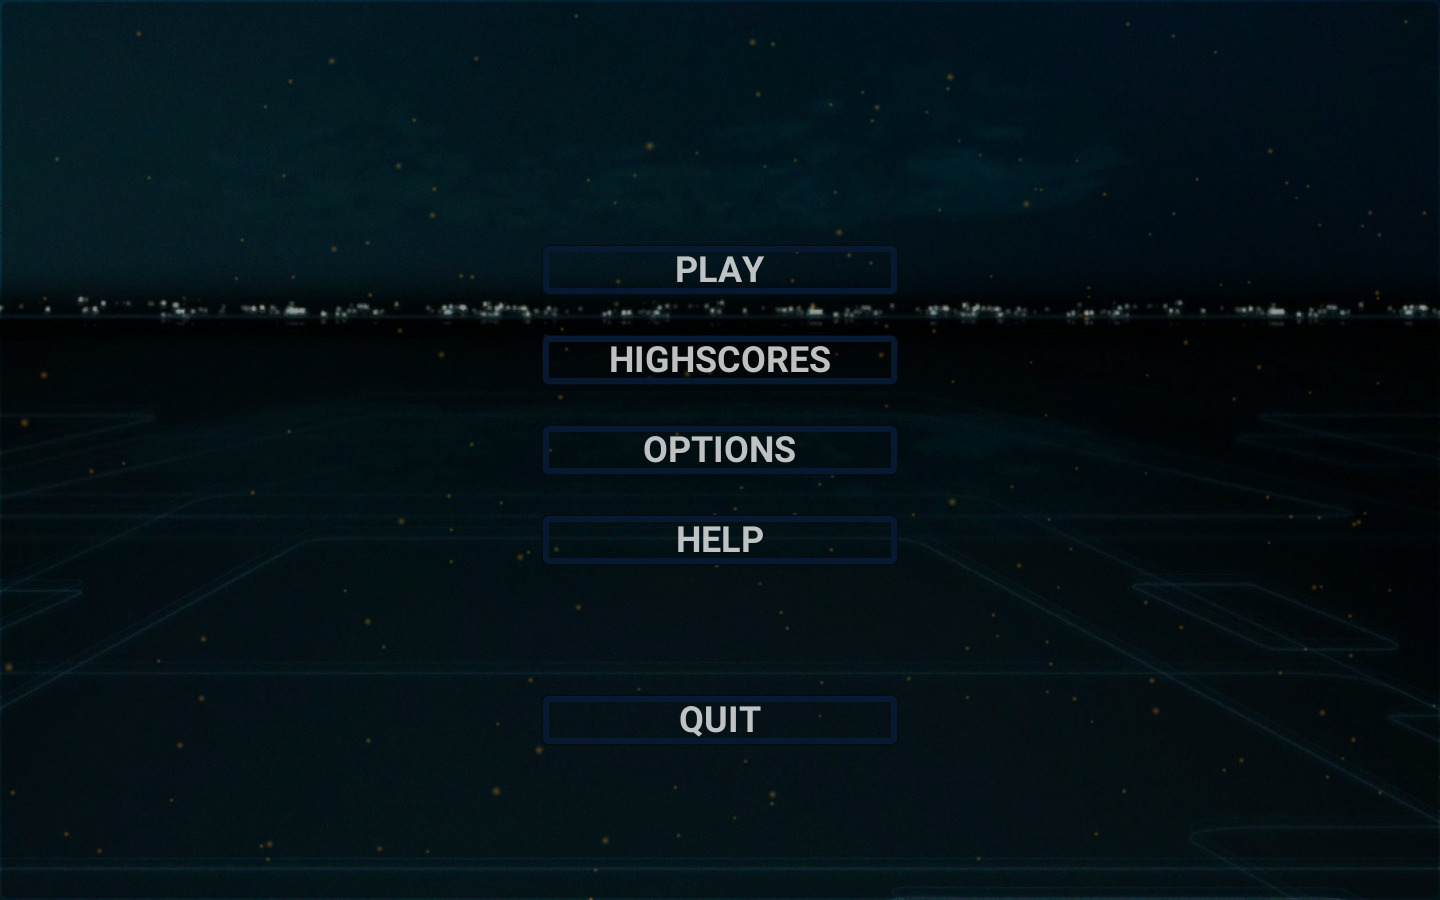
\includegraphics[width=\linewidth]{MainMenu.jpg}
          \caption{Main menu.}
      \end{subfigure}
      \begin{subfigure}[b]{0.33\linewidth}
          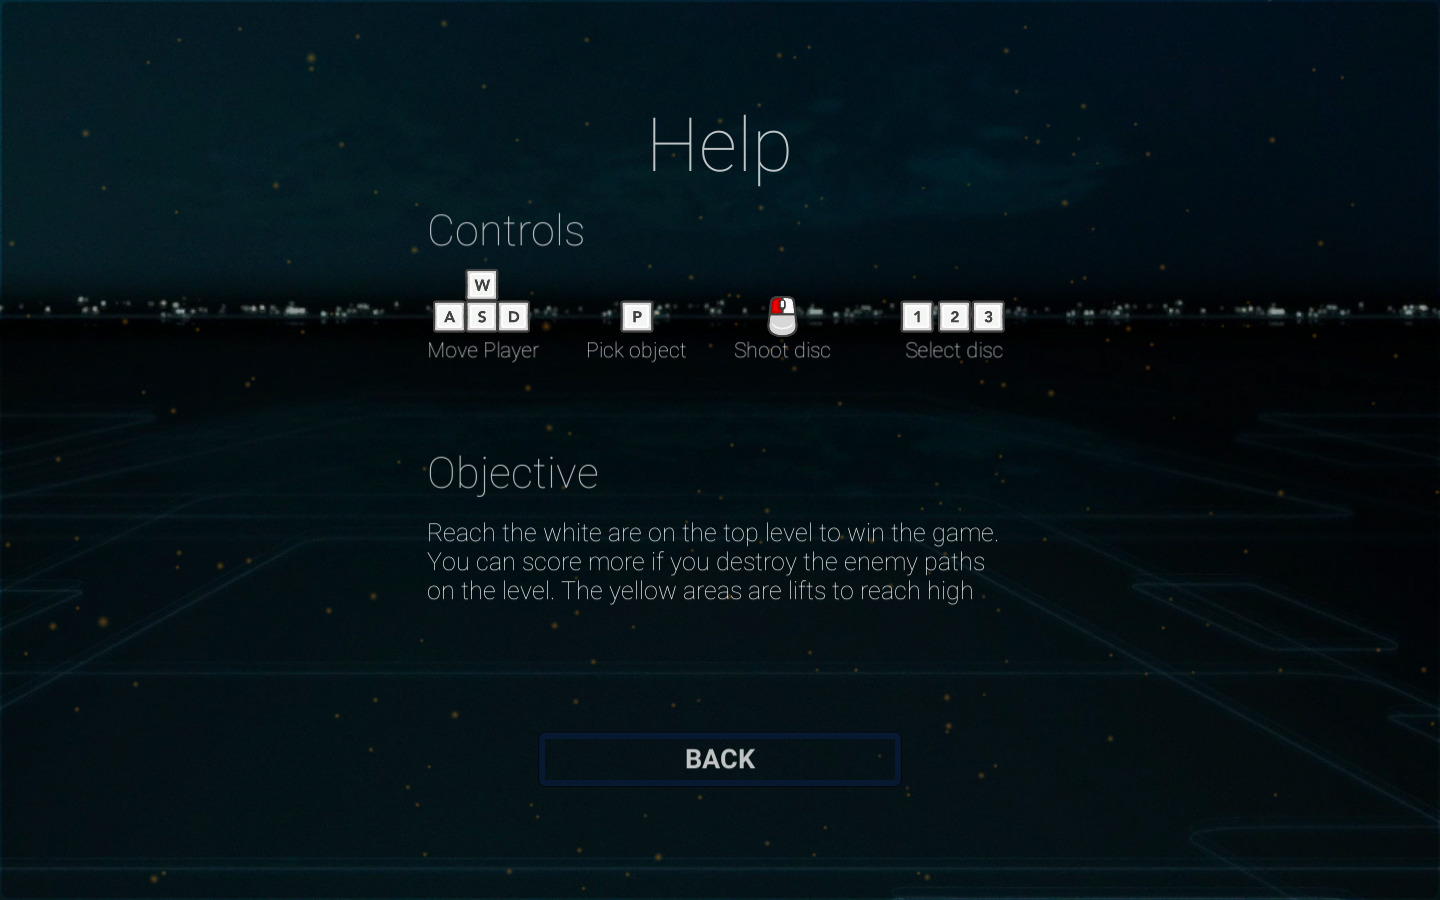
\includegraphics[width=\linewidth]{HelpMenu.jpg}
          \caption{Sub menu.}
      \end{subfigure}
      \begin{subfigure}[b]{0.33\linewidth}
          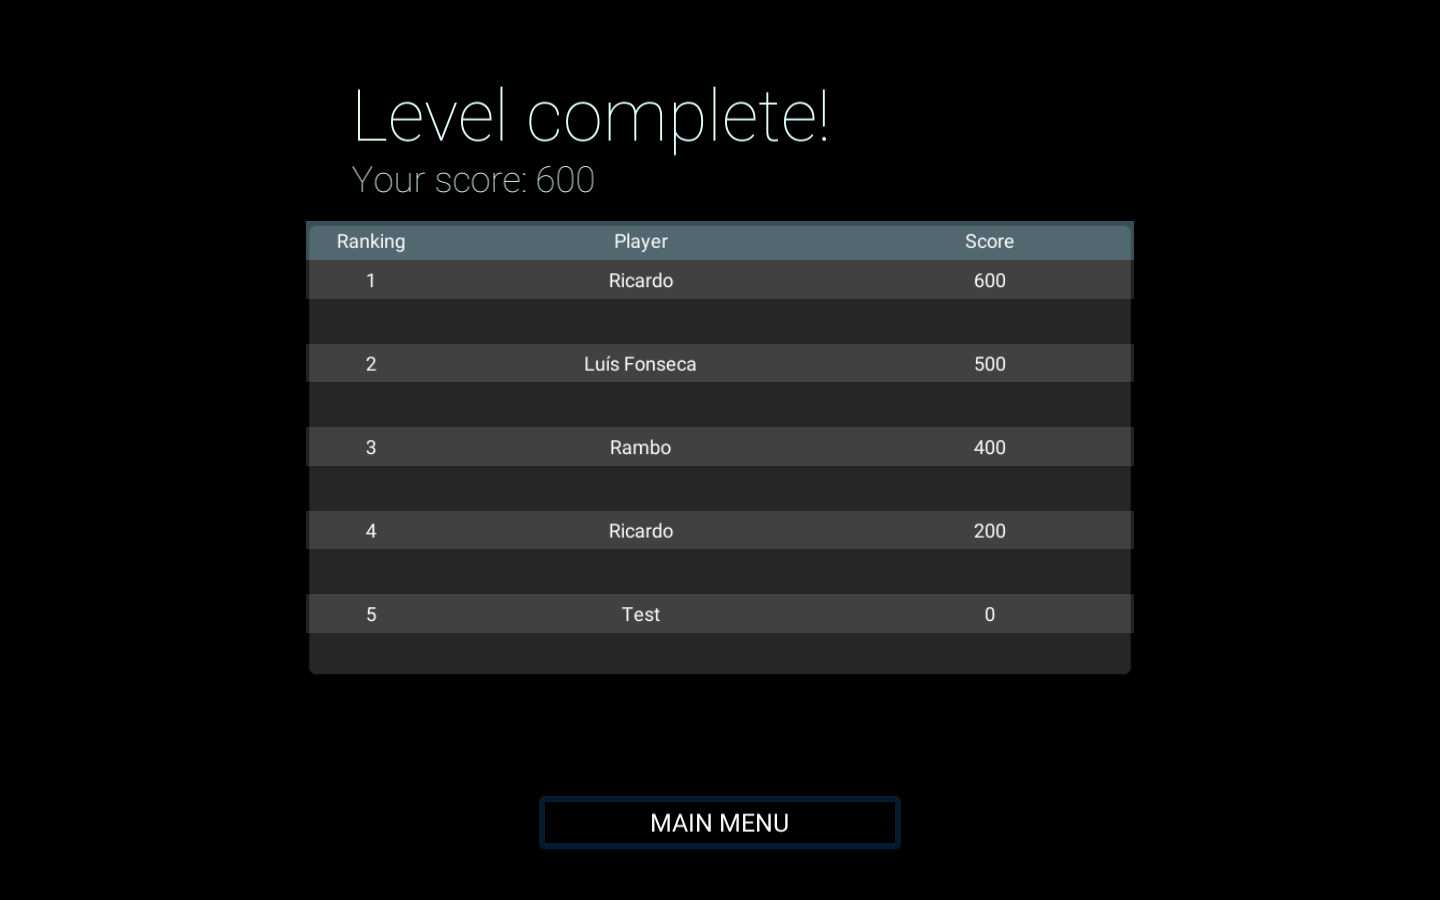
\includegraphics[width=\linewidth]{EndMenu.jpg}
          \caption{End menu.}
      \end{subfigure}
      \caption{Anti-aliasing sampling comparison.}
      \label{fig:animals}
  \end{figure}

  \begin{figure}[H]
      \begin{center}
          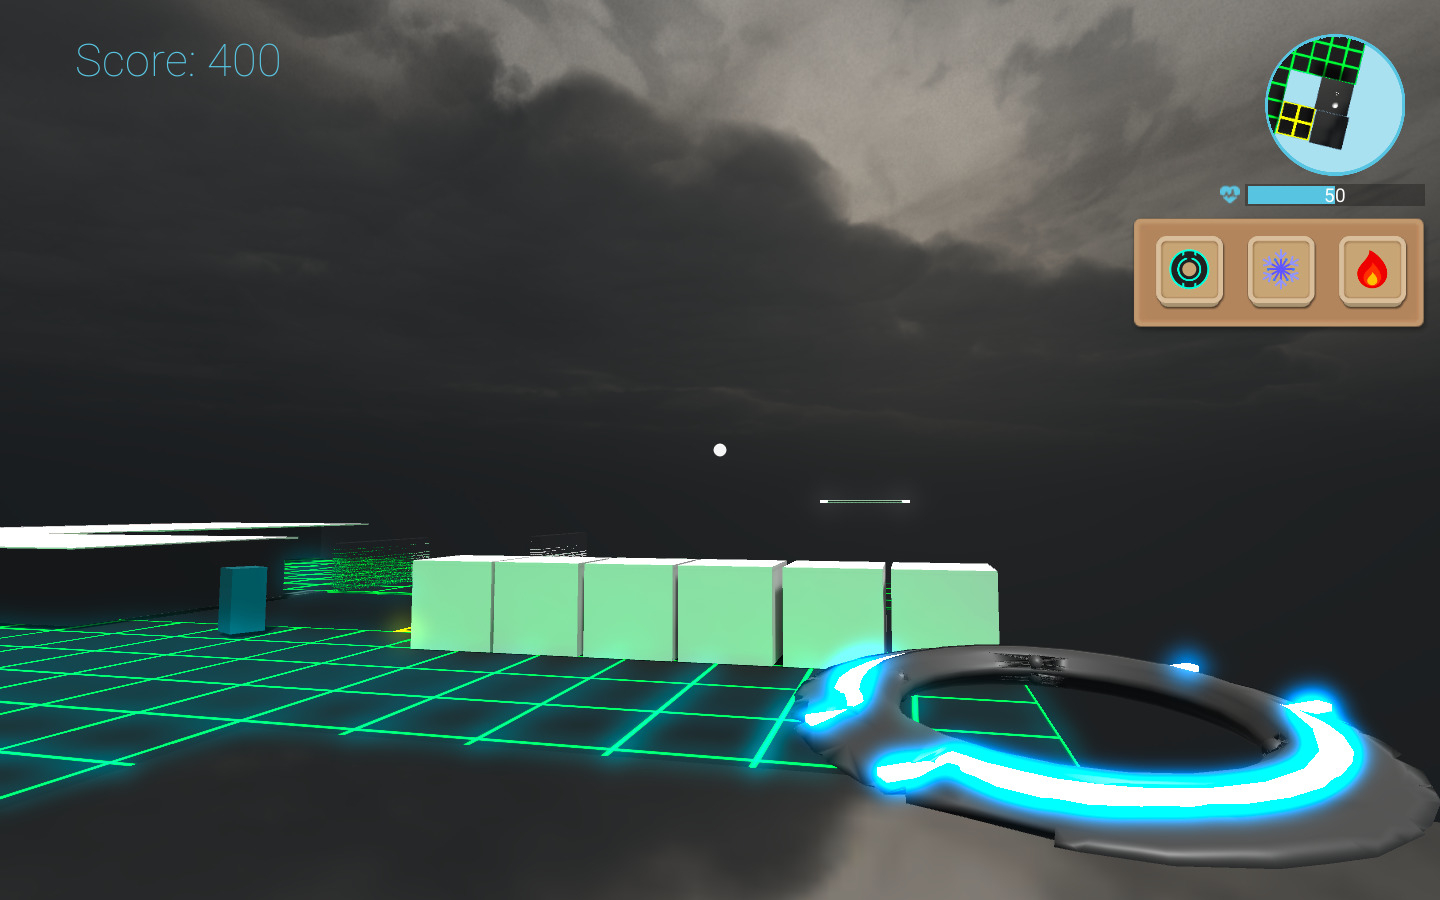
\includegraphics[width=\linewidth]{HUD.jpg}

      \end{center}
      \caption{Heads-Up display containing the current score, a mini map, health bar and the inventory. }
  \end{figure}

\subsection{Visual Effects}
 \begin{figure}[H]
      \begin{subfigure}[b]{0.5\linewidth}
          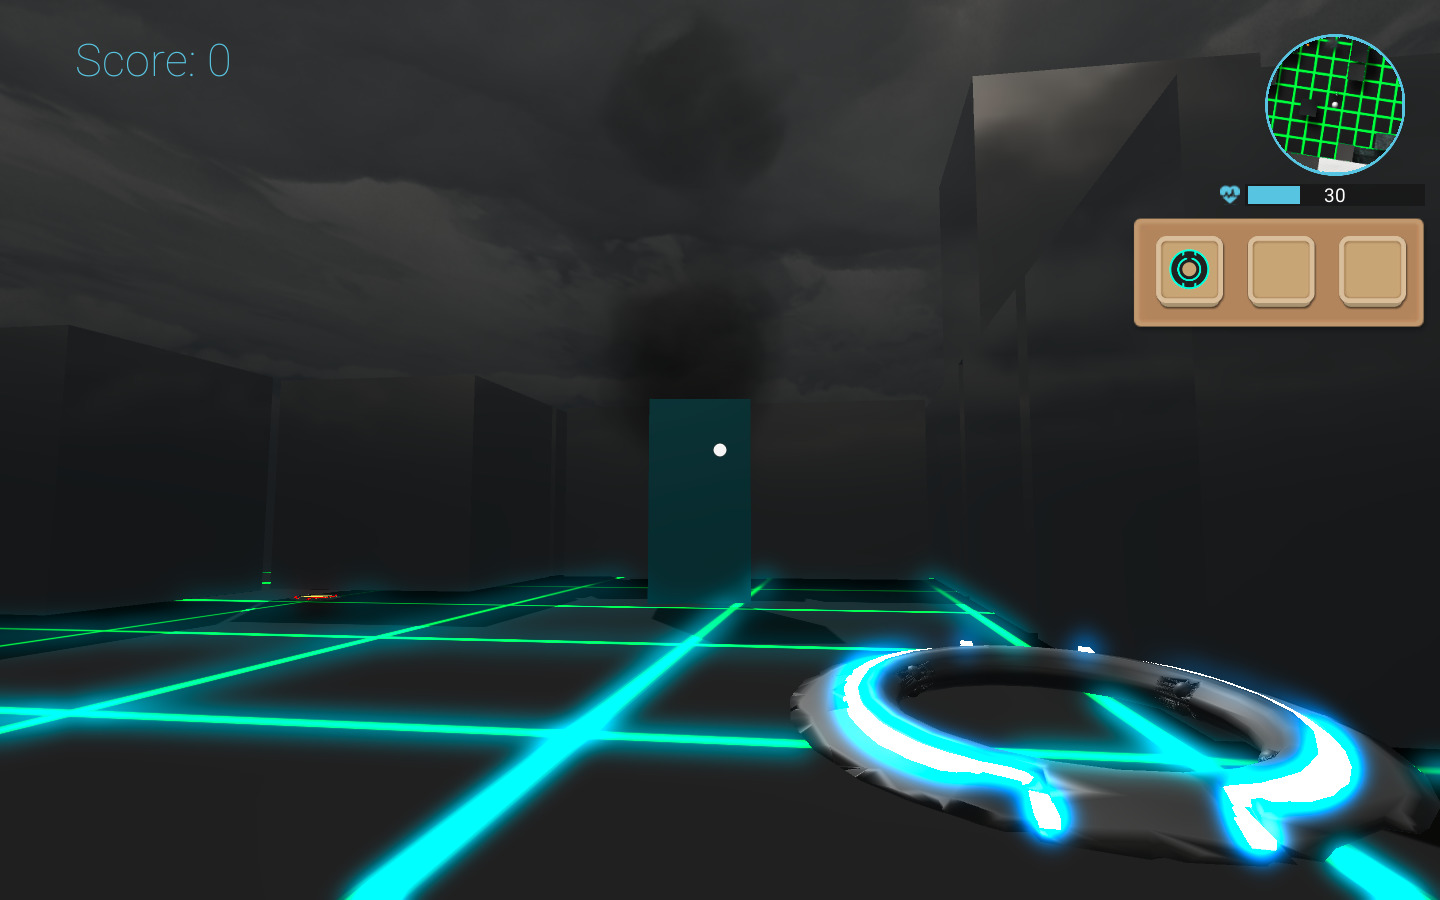
\includegraphics[width=\linewidth]{ParticlesSmoke.jpg}
          \caption{Smoke.}
      \end{subfigure}
      \begin{subfigure}[b]{0.5\linewidth}
          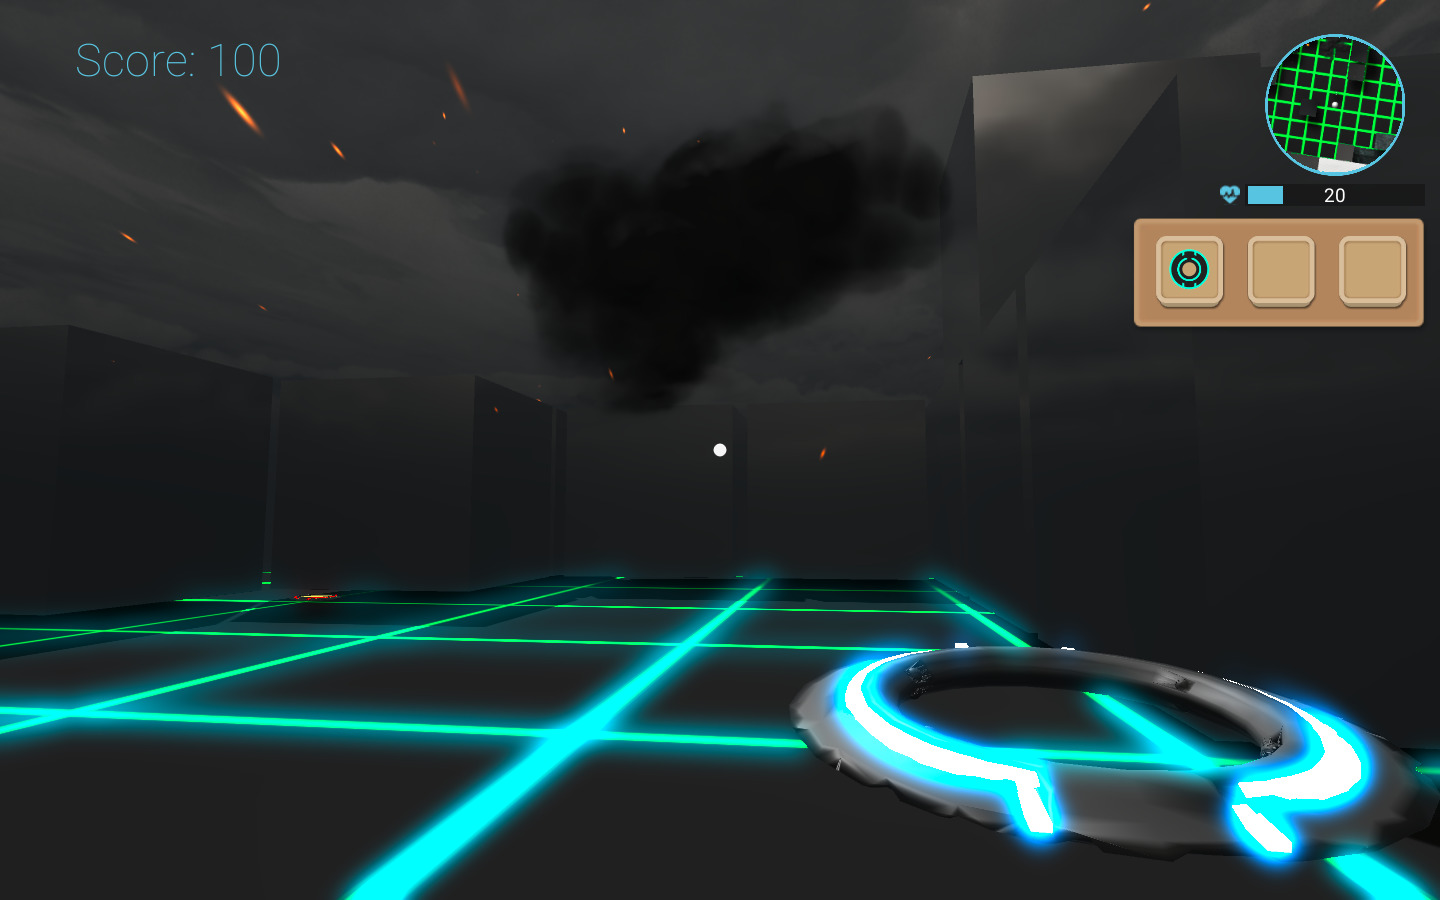
\includegraphics[width=\linewidth]{ParticlesExplosion.jpg}
          \caption{Explosion.}
      \end{subfigure}
      \caption{Particle Systems.}
      \label{fig:particles}
  \end{figure}
  
  \begin{figure}[H]
      \begin{center}
          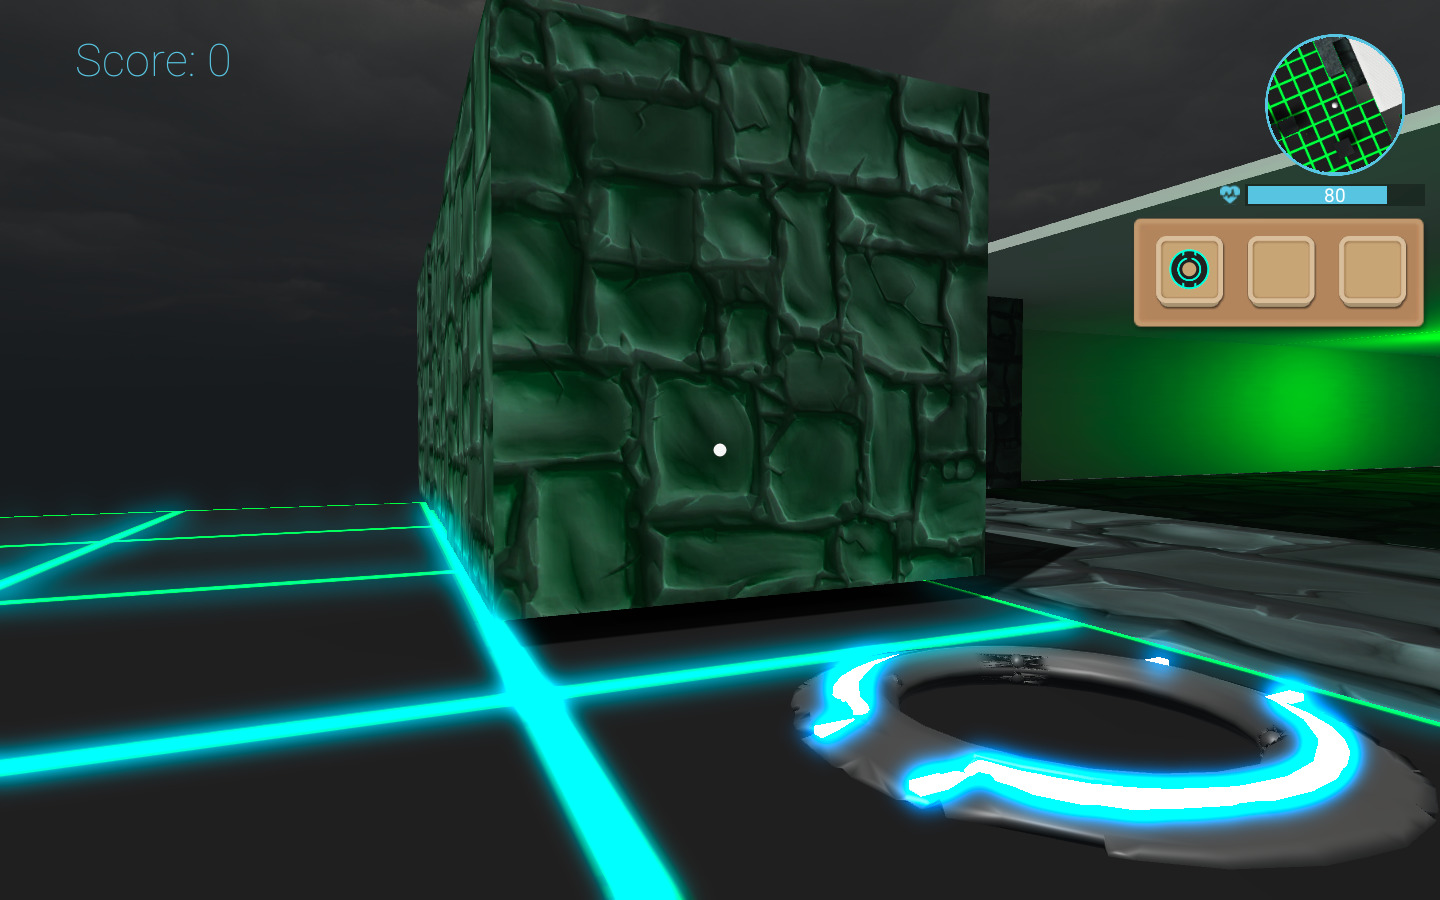
\includegraphics[width=\linewidth]{BumpMapping.jpg}

      \end{center}
      \caption{Stone texture using a normal map.It is also visible shadows obtained from a shadowmap. }
  \end{figure}
    \begin{figure}[H]
      \begin{center}
          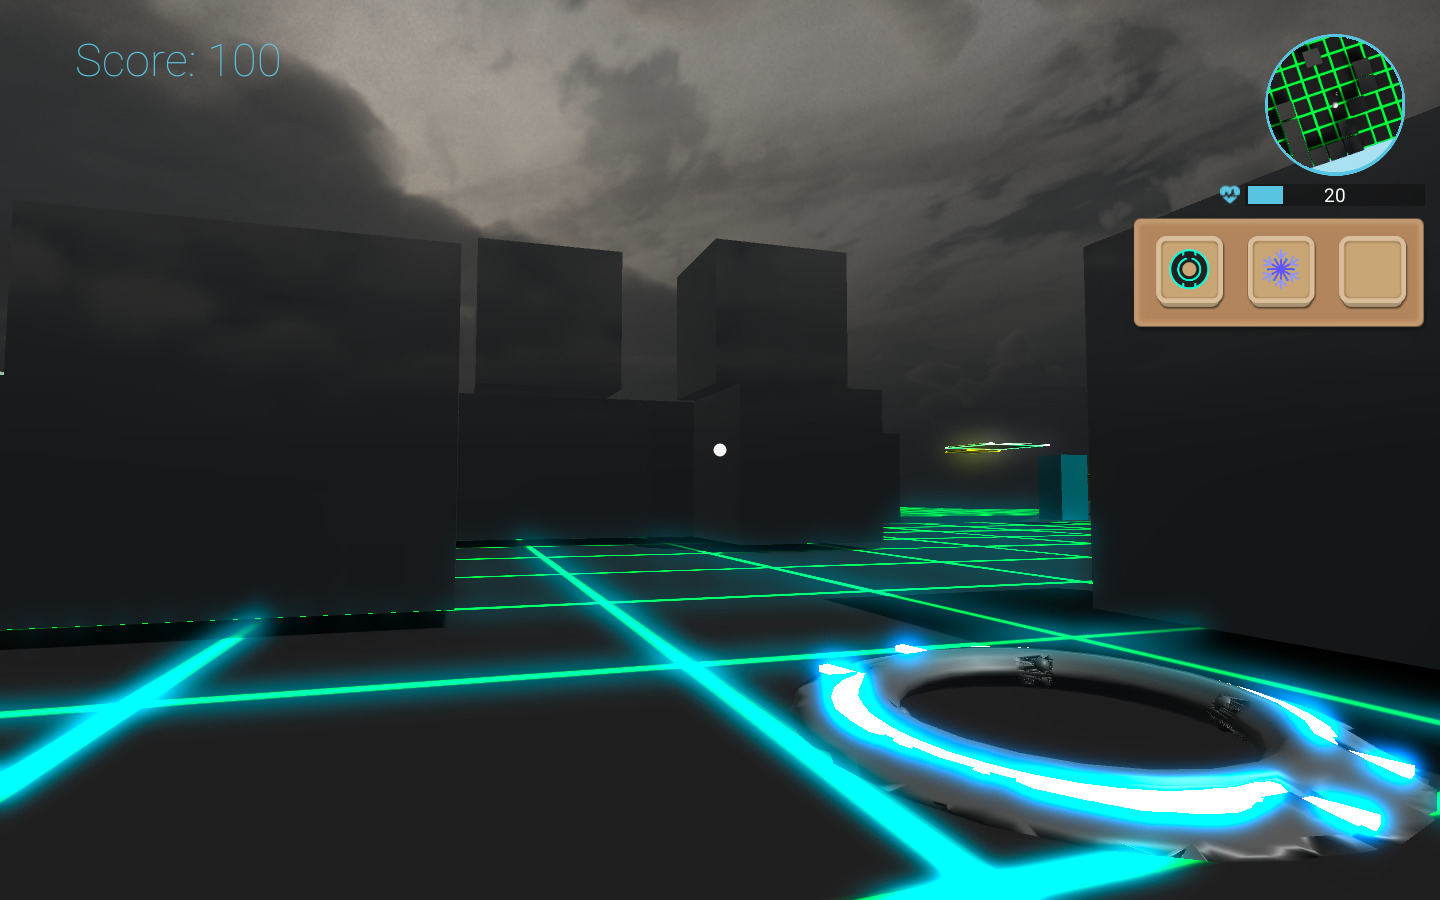
\includegraphics[width=\linewidth]{Bloom.jpg}

      \end{center}
      \caption{HDR Bloom effect in the disc and floor. }
  \end{figure}
    \begin{figure}[H]
      \begin{center}
          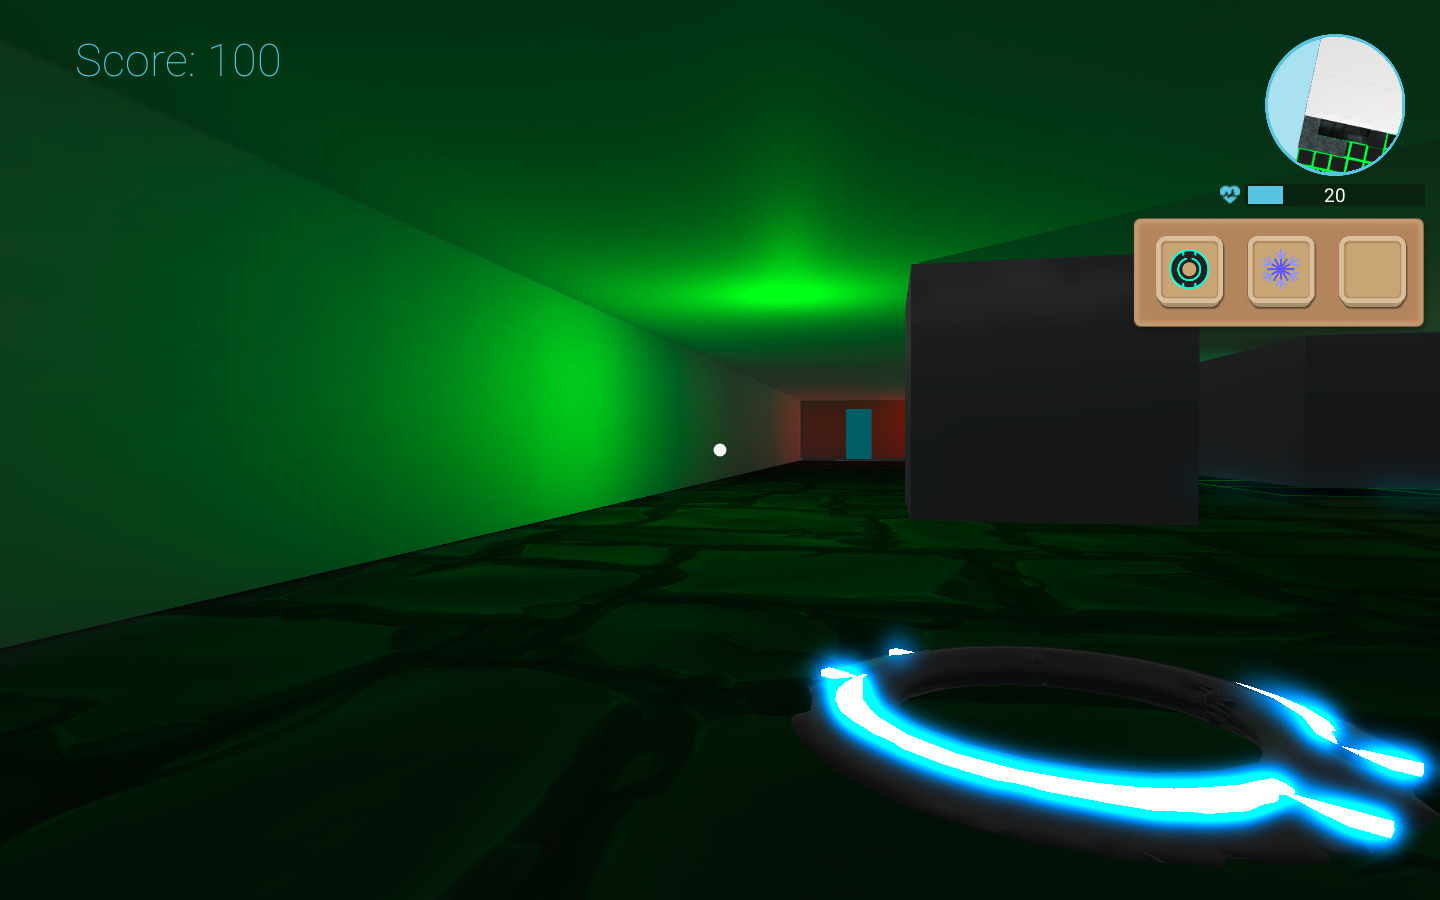
\includegraphics[width=\linewidth]{LightMaps.jpg}

      \end{center}
      \caption{Lightmaps including ambient occlusion. }
  \end{figure}
    \begin{figure}[H]
      \begin{center}
          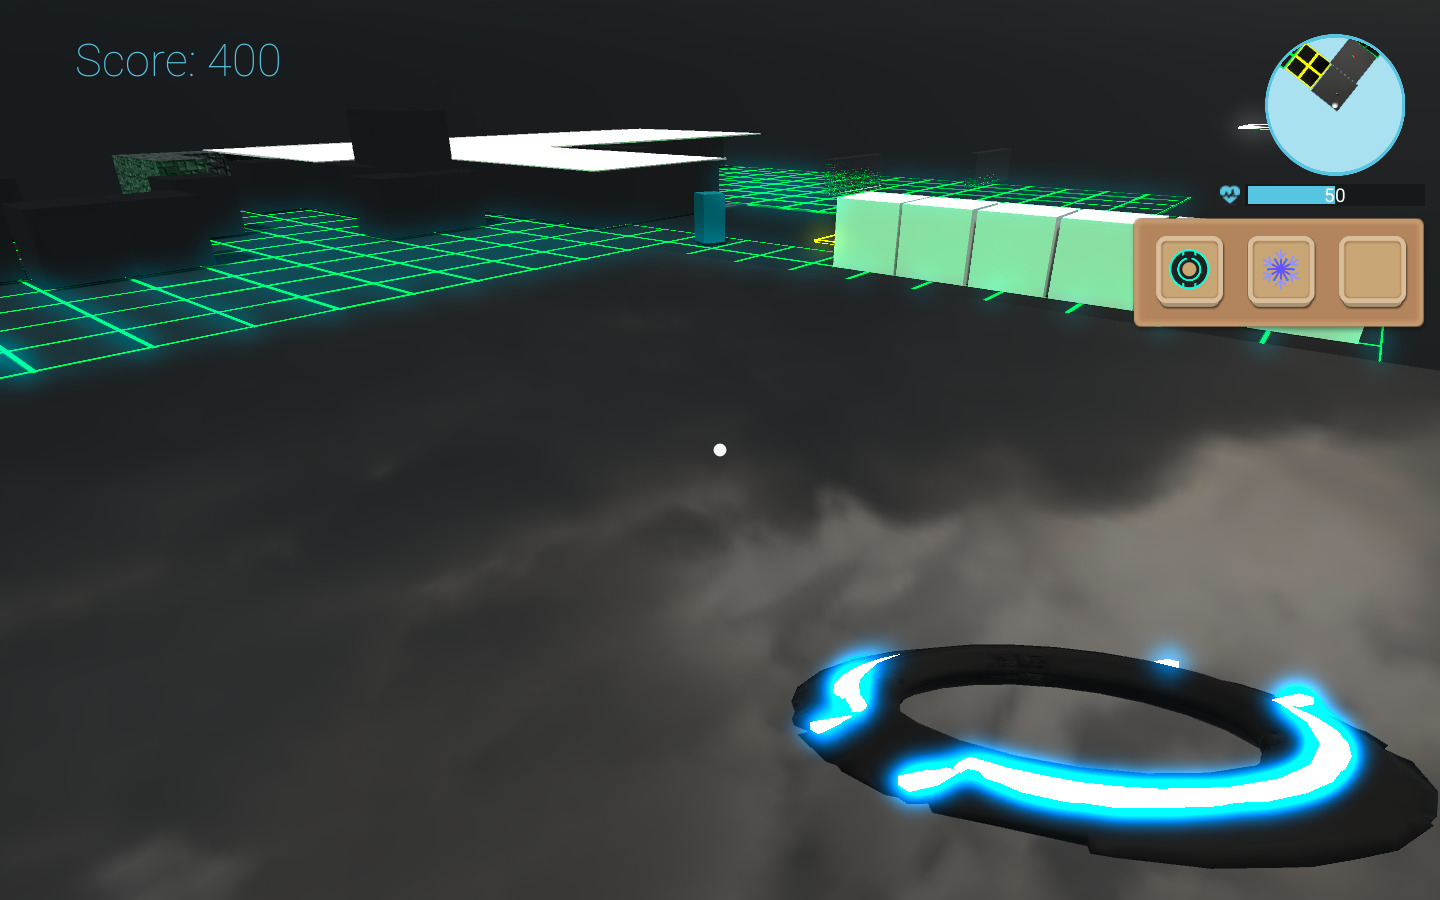
\includegraphics[width=\linewidth]{Reflection.jpg}

      \end{center}
      \caption{Reflections probes. }
  \end{figure}





\newpage
\bibliographystyle{plain}
\bibliography{biblist}


\end{document}